\textbf{Correctness.} We compared all kernels with a float64 reference on eleven shapes covering single tokens ($T{=}S{=}1$), prefill ($T{=}S\in\{7,33,64,100,257,512,1024\}$), chunked prefill against a cache ($T{=}5,S{=}40$; $T{=}128,S{=}300$) and single-token decode against long caches ($T{=}1,S{=}129$), with $H{=}15$, $D{=}64$, batch 1--2 and the offset causal rule. Table~\ref{tab:attnerr} lists the worst-case and mean absolute errors. All fp32 variants and all tile sizes stay below $1.4\times10^{-6}$ and pass \texttt{allclose(atol=1e-5, rtol=1e-4)}; the float64 tiled kernel agrees to $4\times10^{-7}$ (limited by its fp32 inputs' rounding in the comparison). To stress the online softmax we multiplied the queries by 30 (logits in the hundreds): without max-subtraction $e^{s}$ would overflow, but both the explicit reference and the tiled kernel remain finite with the same $5\times10^{-5}$ error, which is the conditioning of the problem in fp32 rather than a kernel bug. Unit tests additionally check that perturbing future keys does not change earlier outputs (causality), and the whole decoder produces the same greedy tokens with \texttt{backend="tiled"} as with SDPA.

\begin{table}[t]\centering\caption{Attention numerical error vs.\ float64 reference (worst / mean over 11 shapes).}\label{tab:attnerr}
\begin{tabular}{lrr}\toprule
Implementation & Max $|\Delta|$ & Mean $|\Delta|$\\\midrule
reference\_fp32 & 1.4e-06 & 3.2e-08 \\
sdpa\_fp32 & 1.4e-06 & 3.1e-08 \\
tiled\_fp32\_b16x16 & 1.3e-06 & 2.9e-08 \\
tiled\_fp32\_b64x64 & 1.3e-06 & 3.0e-08 \\
tiled\_fp32\_b128x64 & 1.3e-06 & 3.0e-08 \\
tiled\_fp64\_b64x64 & 4.1e-07 & 1.2e-08 \\
tiled\_fp32\_b64x64\_scaled30 & 5.0e-05 & 2.9e-07 \\
reference\_fp32\_scaled30 & 5.0e-05 & 2.9e-07 \\
\bottomrule\end{tabular}\end{table}

\textbf{Speed and memory.} Fig.~\ref{fig:attn} and Table~\ref{tab:attnspeed} compare run time (median of 5 after warm-up). With small 64$\times$64 tiles the Python loop issues many tiny matrix products and is 2--4$\times$ \emph{slower} than the explicit reference, and 30$\times$ slower for single-token decode, where there is nothing to tile on the query side. Larger tiles amortise the interpreter overhead: with 256-wide tiles the tiled kernel is faster than the reference from $S{=}512$ on and, at $S{=}2048$, even faster than PyTorch's fused CPU SDPA (252 vs.\ 300\,ms), because it skips the $\approx$50\% of tiles above the causal diagonal while our SDPA call receives a dense boolean mask. The memory advantage is structural: the reference materialises fp32 score and probability matrices of $2HTS\cdot4$ bytes (480\,MB at $T{=}S{=}2048$), whereas the tiled kernel holds one tile (0.5--7.5\,MB). Measured RSS deltas are small and noisy for all kernels because PyTorch's CPU allocator reuses freed blocks between repetitions; we therefore report the analytic sizes as the reliable comparison. On GPUs a fused kernel such as FlashAttention also wins on speed because it keeps tiles in on-chip SRAM and fuses the exponentials and matrix products into one kernel launch; an educational PyTorch implementation cannot control memory placement, launches several operations per tile and runs the loop in Python, so it should not be expected to beat a fused kernel in general.

\begin{figure}[t]\centering
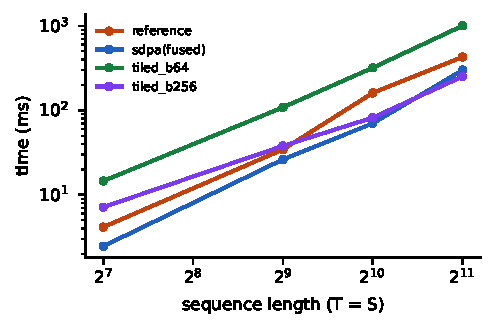
\includegraphics[width=\columnwidth]{figures/attn_speed.pdf}
\caption{Causal attention time for $T{=}S$ (15 heads, $D{=}64$, fp32, 10 CPU threads). Tiled performance depends strongly on tile size.}\label{fig:attn}
\end{figure}

\begin{table}[t]\centering\caption{Attention timing (ms, median of 5) and memory (peak RSS delta and analytic largest intermediate, MB).}\label{tab:attnspeed}
\setlength{\tabcolsep}{3pt}\footnotesize
\begin{tabular}{rrlrrr}\toprule
$T$ & $S$ & Impl. & ms & $\Delta$RSS & Interm.\\\midrule
128 & 128 & reference & 4.14 & 0.4 & 1.88 \\
128 & 128 & sdpa(fused) & 2.46 & 0.1 & fused \\
128 & 128 & tiled\_b64 & 14.56 & 0.1 & 0.47 \\
128 & 128 & tiled\_b128 & 6.90 & 1.0 & 1.88 \\
128 & 128 & tiled\_b256 & 7.14 & 1.0 & 1.88 \\
512 & 512 & reference & 34.40 & 4.0 & 30.00 \\
512 & 512 & sdpa(fused) & 26.22 & 0.1 & fused \\
512 & 512 & tiled\_b64 & 108.49 & 0.0 & 0.47 \\
512 & 512 & tiled\_b128 & 57.84 & 0.0 & 1.88 \\
512 & 512 & tiled\_b256 & 37.91 & 0.0 & 7.50 \\
1024 & 1024 & reference & 160.77 & 0.0 & 120.00 \\
1024 & 1024 & sdpa(fused) & 70.10 & 5.7 & fused \\
1024 & 1024 & tiled\_b64 & 319.28 & 3.8 & 0.47 \\
1024 & 1024 & tiled\_b128 & 133.62 & 0.8 & 1.88 \\
1024 & 1024 & tiled\_b256 & 81.88 & 0.0 & 7.50 \\
2048 & 2048 & reference & 428.78 & 0.0 & 480.00 \\
2048 & 2048 & sdpa(fused) & 299.58 & 5.7 & fused \\
2048 & 2048 & tiled\_b64 & 1003.66 & 8.0 & 0.47 \\
2048 & 2048 & tiled\_b128 & 395.49 & 0.0 & 1.88 \\
2048 & 2048 & tiled\_b256 & 251.57 & 0.1 & 7.50 \\
1 & 1024 & reference & 2.06 & 0.0 & 0.12 \\
1 & 1024 & sdpa(fused) & 0.84 & 0.0 & fused \\
1 & 1024 & tiled\_b64 & 27.13 & 0.0 & 0.01 \\
1 & 1024 & tiled\_b128 & 9.53 & 0.0 & 0.01 \\
1 & 1024 & tiled\_b256 & 8.18 & 0.0 & 0.03 \\
1 & 4096 & reference & 4.65 & 0.0 & 0.47 \\
1 & 4096 & sdpa(fused) & 1.24 & 0.1 & fused \\
1 & 4096 & tiled\_b64 & 30.58 & 0.0 & 0.01 \\
1 & 4096 & tiled\_b128 & 20.82 & 0.0 & 0.01 \\
1 & 4096 & tiled\_b256 & 11.44 & 0.0 & 0.03 \\
64 & 2048 & reference & 11.55 & 0.0 & 15.00 \\
64 & 2048 & sdpa(fused) & 11.90 & 0.0 & fused \\
64 & 2048 & tiled\_b64 & 33.85 & 0.0 & 0.47 \\
64 & 2048 & tiled\_b128 & 29.43 & 0.0 & 0.94 \\
64 & 2048 & tiled\_b256 & 19.20 & 0.0 & 1.88 \\
\bottomrule\end{tabular}\end{table}
